\documentclass[10pt]{article}
\usepackage[margin=1.0cm]{geometry}
\usepackage[T1]{fontenc}
\usepackage{lmodern}
\usepackage{xcolor}
\usepackage{tikz}
\usepackage{pgfplots}
\usepgfplotslibrary{statistics}
\pgfplotsset{compat=1.18}
\definecolor{srblue}{HTML}{2F6B9A}
\definecolor{opencvorange}{HTML}{D97706}
\definecolor{fps2blue}{HTML}{B9D7EA}
\definecolor{fps5orange}{HTML}{F6C28B}
\definecolor{stslightgreen}{HTML}{A7D8B1}
\definecolor{stsstronggreen}{HTML}{208B3A}
\definecolor{sugarlightpurple}{HTML}{CBB7E8}
\definecolor{sugarstrongpurple}{HTML}{763A9B}
\definecolor{stsedge}{HTML}{1D4E89}
\definecolor{sugaredge}{HTML}{B45309}
\definecolor{incompletegray}{HTML}{9CA3AF}
\definecolor{deltared}{HTML}{B91C1C}
\definecolor{deltagreen}{HTML}{15803D}
\begin{document}
\pagestyle{empty}
\begin{center}
{\Large\bfseries STS: gemittelte objektmaskierte Bildmetriken}\\[3pt]
{\small Mittelwerte aus historischen und Repeat-Läufen}\\[8pt]
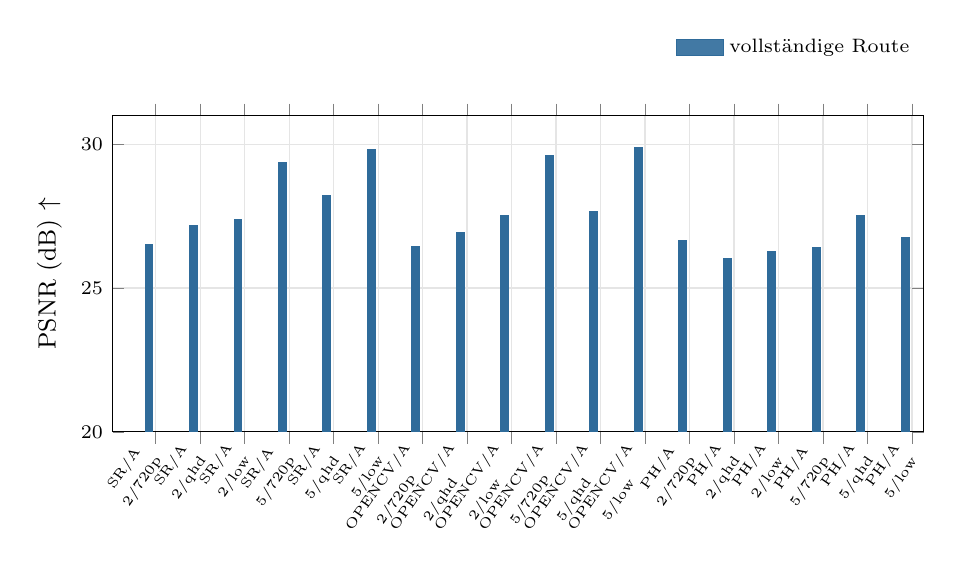
\begin{tikzpicture}
\begin{axis}[height=5.6cm,width=0.98\linewidth,ybar,bar width=2.8pt,enlarge x limits=0.015,xmin=-0.7,ymin=20,ymax=31,xtick=data,xticklabels={{\shortstack{SR/A\\2/720p}},{\shortstack{SR/A\\2/qhd}},{\shortstack{SR/A\\2/low}},{\shortstack{SR/A\\5/720p}},{\shortstack{SR/A\\5/qhd}},{\shortstack{SR/A\\5/low}},{\shortstack{OPENCV/A\\2/720p}},{\shortstack{OPENCV/A\\2/qhd}},{\shortstack{OPENCV/A\\2/low}},{\shortstack{OPENCV/A\\5/720p}},{\shortstack{OPENCV/A\\5/qhd}},{\shortstack{OPENCV/A\\5/low}},{\shortstack{PH/A\\2/720p}},{\shortstack{PH/A\\2/qhd}},{\shortstack{PH/A\\2/low}},{\shortstack{PH/A\\5/720p}},{\shortstack{PH/A\\5/qhd}},{\shortstack{PH/A\\5/low}}},x tick label style={font=\tiny,rotate=55,anchor=east},ylabel style={font=\small},tick label style={font=\scriptsize},ylabel={PSNR (dB) $\uparrow$},grid=major,grid style={gray!20},legend style={font=\scriptsize,at={(1.0,1.15)},anchor=south east,draw=none,fill=white,fill opacity=0.9,text opacity=1},xtick={0,1,2,3,4,5,6,7,8,9,10,11,12,13,14,15,16,17}]
\addplot+[fill=srblue,draw=srblue,area legend] coordinates {(0,26.50121269) (1,27.18327996) (2,27.38534741) (3,29.36834851) (4,28.20878513) (5,29.81829738) (6,26.45132990) (7,26.91983874) (8,27.53341959) (9,29.61294152) (10,27.66550179) (11,29.89049716) (12,26.64421298) (13,26.02053897) (14,26.25806929) (15,26.39010134) (16,27.51721004) (17,26.73754651)};
\addlegendentry{vollständige Route}
\addplot+[fill=incompletegray,draw=incompletegray,area legend] coordinates {};
\addlegendentry{STS-Zwischenmetrik unvollständiger Route}
\end{axis}
\end{tikzpicture}
\par\vspace{2pt}
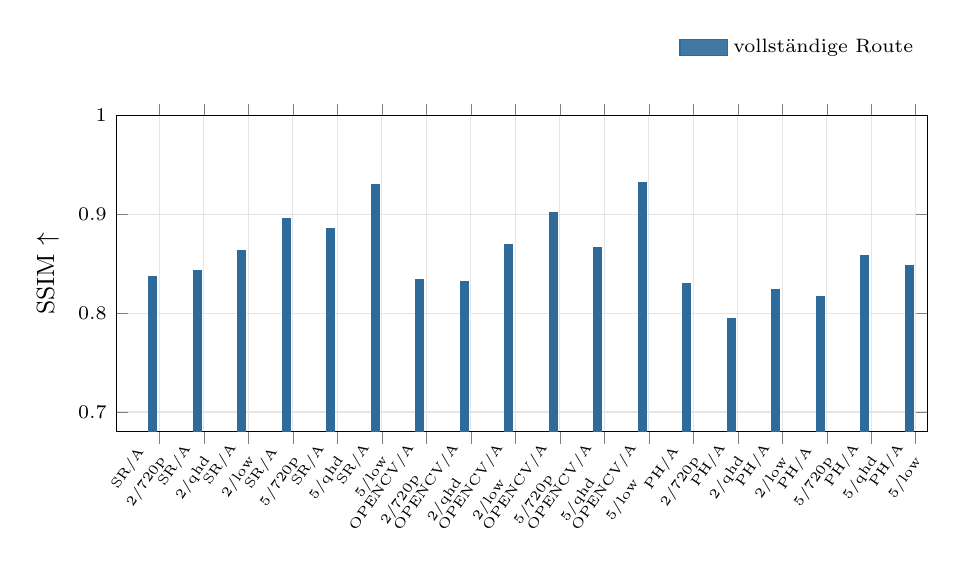
\begin{tikzpicture}
\begin{axis}[height=5.6cm,width=0.98\linewidth,ybar,bar width=2.8pt,enlarge x limits=0.015,xmin=-0.7,ymin=0.68,ymax=1.0,xtick=data,xticklabels={{\shortstack{SR/A\\2/720p}},{\shortstack{SR/A\\2/qhd}},{\shortstack{SR/A\\2/low}},{\shortstack{SR/A\\5/720p}},{\shortstack{SR/A\\5/qhd}},{\shortstack{SR/A\\5/low}},{\shortstack{OPENCV/A\\2/720p}},{\shortstack{OPENCV/A\\2/qhd}},{\shortstack{OPENCV/A\\2/low}},{\shortstack{OPENCV/A\\5/720p}},{\shortstack{OPENCV/A\\5/qhd}},{\shortstack{OPENCV/A\\5/low}},{\shortstack{PH/A\\2/720p}},{\shortstack{PH/A\\2/qhd}},{\shortstack{PH/A\\2/low}},{\shortstack{PH/A\\5/720p}},{\shortstack{PH/A\\5/qhd}},{\shortstack{PH/A\\5/low}}},x tick label style={font=\tiny,rotate=55,anchor=east},ylabel style={font=\small},tick label style={font=\scriptsize},ylabel={SSIM $\uparrow$},grid=major,grid style={gray!20},legend style={font=\scriptsize,at={(1.0,1.15)},anchor=south east,draw=none,fill=white,fill opacity=0.9,text opacity=1},xtick={0,1,2,3,4,5,6,7,8,9,10,11,12,13,14,15,16,17}]
\addplot+[fill=srblue,draw=srblue,area legend] coordinates {(0,0.83657259) (1,0.84303451) (2,0.86367902) (3,0.89594813) (4,0.88555103) (5,0.93023792) (6,0.83392095) (7,0.83151061) (8,0.86978696) (9,0.90148111) (10,0.86666241) (11,0.93208752) (12,0.83034673) (13,0.79501773) (14,0.82414792) (15,0.81667582) (16,0.85779472) (17,0.84843206)};
\addlegendentry{vollständige Route}
\addplot+[fill=incompletegray,draw=incompletegray,area legend] coordinates {};
\addlegendentry{STS-Zwischenmetrik unvollständiger Route}
\end{axis}
\end{tikzpicture}
\par\vspace{2pt}
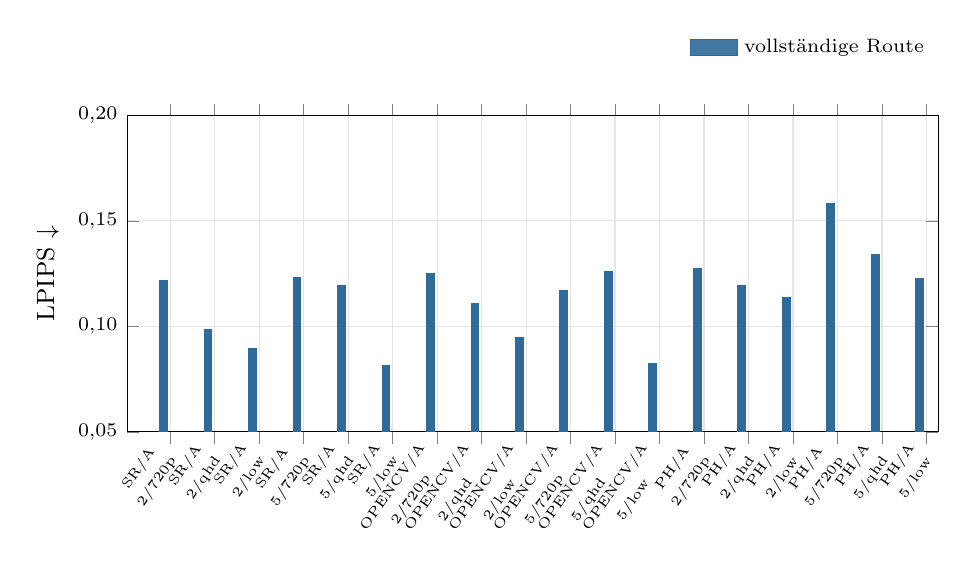
\begin{tikzpicture}
\begin{axis}[height=5.6cm,width=0.98\linewidth,ybar,bar width=2.8pt,enlarge x limits=0.015,xmin=-0.7,ymin=0.05,ymax=0.2,xtick=data,xticklabels={{\shortstack{SR/A\\2/720p}},{\shortstack{SR/A\\2/qhd}},{\shortstack{SR/A\\2/low}},{\shortstack{SR/A\\5/720p}},{\shortstack{SR/A\\5/qhd}},{\shortstack{SR/A\\5/low}},{\shortstack{OPENCV/A\\2/720p}},{\shortstack{OPENCV/A\\2/qhd}},{\shortstack{OPENCV/A\\2/low}},{\shortstack{OPENCV/A\\5/720p}},{\shortstack{OPENCV/A\\5/qhd}},{\shortstack{OPENCV/A\\5/low}},{\shortstack{PH/A\\2/720p}},{\shortstack{PH/A\\2/qhd}},{\shortstack{PH/A\\2/low}},{\shortstack{PH/A\\5/720p}},{\shortstack{PH/A\\5/qhd}},{\shortstack{PH/A\\5/low}}},x tick label style={font=\tiny,rotate=55,anchor=east},ylabel style={font=\small},tick label style={font=\scriptsize},ylabel={LPIPS $\downarrow$},grid=major,grid style={gray!20},scaled y ticks=false,ytick={0.05,0.10,0.15,0.20},yticklabels={{0,05},{0,10},{0,15},{0,20}},legend style={font=\scriptsize,at={(1.0,1.15)},anchor=south east,draw=none,fill=white,fill opacity=0.9,text opacity=1},xtick={0,1,2,3,4,5,6,7,8,9,10,11,12,13,14,15,16,17}]
\addplot+[fill=srblue,draw=srblue,area legend] coordinates {(0,0.12185202) (1,0.09865326) (2,0.08929665) (3,0.12320841) (4,0.11937699) (5,0.08152318) (6,0.12505824) (7,0.11104393) (8,0.09456848) (9,0.11720216) (10,0.12601008) (11,0.08239057) (12,0.12737379) (13,0.11923454) (14,0.11378294) (15,0.15818454) (16,0.13414868) (17,0.12262199)};
\addlegendentry{vollständige Route}
\addplot+[fill=incompletegray,draw=incompletegray,area legend] coordinates {};
\addlegendentry{STS-Zwischenmetrik unvollständiger Route}
\end{axis}
\end{tikzpicture}
\par\vspace{2pt}
\vspace{3pt}
\begin{minipage}{0.98\linewidth}\scriptsize Dargestellt werden ausschließlich vollständige Original-GS-A-Routen. Vorhandene \texttt{sts\_masked.json}-Dateien aus später fehlgeschlagenen SuGaR-Routen bleiben als Fehlernachweis archiviert, werden hier aber nicht zusätzlich dargestellt. Die Auswertung ist objektmaskiert; die Werte stammen aus der jeweiligen Runauflösung.\end{minipage}
\end{center}
\end{document}